\section{Energy-Efficient Networks}
\label{EEN}
%wireless sensor networks: duty circle 
In an energy-efficient network (i.e., wireless sensor networks), 
the battery-consumption is a crucial factor to be taken into account.
Duty circle is a key technique to deal with the dilemma between a 
balance of energy-efficiency and low-latency.


%the structure of the rest part in this section
We first consider the homogenous energy-arrangement situation
that  all the nodes share a global duty circle $\theta$, and propose
a RDS based Alano algorithm. Then we propose a traversing pointer 
based Alano algorithm for a more general scenario, 
where nodes have heterogeneous battery-scheduling 
capability with local duty circle $\theta_i$.

%an overview of the motivation of the algorithm
Our initiative idea is to align the wake-up slots of the neighbor nodes within a bounded time,
and then invoke the Alano algorithm to achieve neighbor discovery process w.h.p. 
More specifically, we utilize the property of RDS and traversing pointer to guarantee 
a wake-up slot rendezvous in each period $T$. 

\subsection{Global $\theta$: A RDS Based Alano Algorithm}

%Consider Global Duty Circle
When a global duty circle $\theta$ is shared by all the nodes in the network,
we utilize relaxed difference set (RDS) to align the wake-up time slots.


%Introduction of RDS and the property
%*High coincidence of another existing paper && to be altered later
Relaxed difference set (RDS) is an efficient tool to 
construct cyclic quorum systems\cite{jiang2005quorum,luk1997two}. The definition can be
described as:
\begin{definition}
A set $R=\{a_1,a_2,...,a_k\} \subseteq Z_n$ (the set of all nonnegative integers less than $n$) 
is called a Relaxed Difference Set (RDS) if for every $d \neq 0$ (mod $n$), 
there exists at least one ordered pair $(a_i,a_j)$ such that $a_i - a_j \equiv d$ (mod $n$), where $a_i,a_j \in D$.
\end{definition}

It has been proved that 
any RDS must have cardinality $|R| \geq \sqrt{N}$\cite{luk1997two}.
We present a simple linear algorithm for RDS construction under $Z_N$
with$\lceil \frac{3\sqrt{N}}{2}  \rceil$ cardinality in Alg. \ref{RDS}. 
%*High coincidence

%RDS construction
\begin{algorithm}
\caption{RDS construction under $Z_N$}
\label{RDS}
\begin{algorithmic}[1]
\STATE $R :=\emptyset$;
\STATE $\lambda :=\lceil \sqrt{N}  \rceil$,$\mu :=\lceil \frac{\lceil \sqrt{N} \rceil}{2} \rceil$;\label{RDSline1}
\FOR{$i = 1 :\lambda$}
	\STATE $R :=R \cup i$; \label{RDSline2}
\ENDFOR
\FOR{$j = 1 :\mu$}
	\STATE $R :=R \cup (1 + j * \lambda )$; \label{RDSline3}
\ENDFOR
\end{algorithmic}
\end{algorithm}


The initiative idea of Alg. \ref{RDS} can be described as Fig. \ref{matrix}. 
The framed elements are selected as in Alg. \ref{RDS} 
Line. \ref{RDSline2} and Line. \ref{RDSline3}. 

\begin{figure}[htb]
\centering
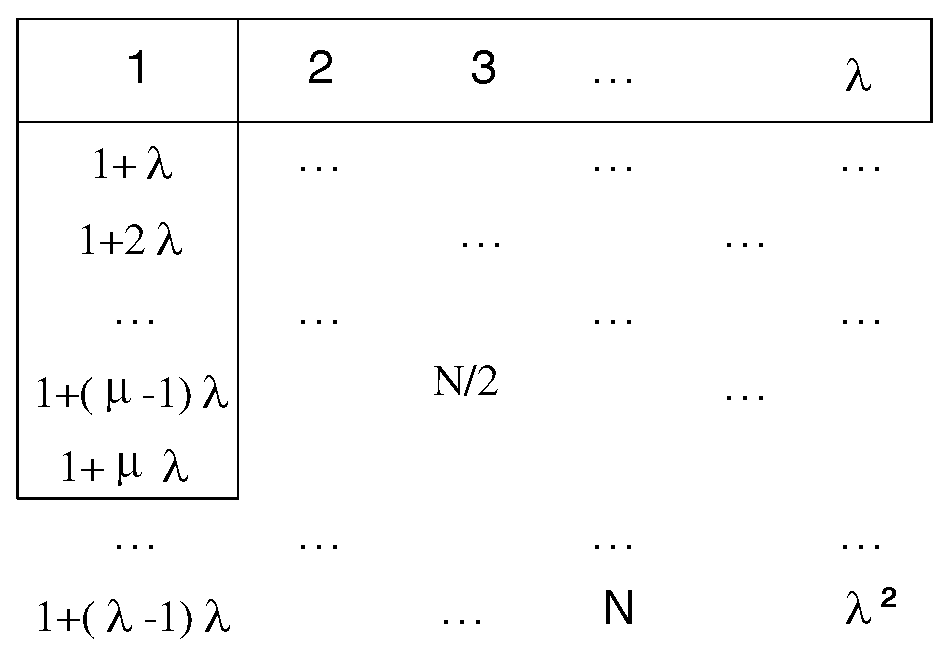
\includegraphics[width=2in]{./Figure/matrix}
\caption{An Sketch of RDS construction in Alg. \ref{RDS}}
\label{matrix}
\end{figure}

We give a formal correctness proof of the construction as following:

%The correctness proof of the construction
\begin{theorem}
\label{RDS1}
The set $R = \{r_0, r_1, ..., r_{\lambda + \mu - 1}\}$ constructed in Alg. \ref{RDS} is a RDS,
where $|R| = \lambda + \mu = \lceil \sqrt{N}  \rceil + \lceil \frac{\lceil \sqrt{N} \rceil}{2} \rceil
\approx \lceil \frac{3\sqrt{N}}{2}  \rceil$.
\end{theorem}


\begin{IEEEproof}
We first reach a consensus that if there exists one ordered 
pair $(a_i,a_j)$ satisfying  $a_i - a_j \equiv d$ (mod $N$),
then we can get an opposite pair $(a_j,a_i)$ such that  
$a_j - a_i \equiv (N-d)$ (mod $n$). Thus we only need to find 
at least one ordered pair $(a_i,a_j)$ for each $d$ from $1$ to $\lfloor N/2 \rfloor$.

The $\lambda$ in Line \ref{RDSline1} is the smallest integer satisfying 
$\lambda^2 \geq N$. Then every $d$ from $1$ to $\lfloor N/2 \rfloor$ 
can be represented as: $ d = 1 + j \times \lambda - i$, where $1 \leq j \leq \mu, 
1 \leq i \leq \lambda$. Thus there exists $a_j = 1 + j \times \lambda$ 
added in Line. \ref{RDSline2} and $a_i = i$ added in Line. \ref{RDSline3} 
satisfying  $a_j - a_i \equiv d$.
\end{IEEEproof}


%RDS Based Alano Algorithm

Next, we present a RDS based Alano algorithm (RDS-Alano) in Alg. \ref{RDS-ND},
to achieve neighbor discovery process in a partially-connected
and energy-efficient network with global duty circle $\theta$. 

In Alg. \ref{RDS-ND}, RDS is used to construct a deterministic 
schedule for the node to wake up in every period $T$, 
and Alano is utilized as a probabilistic strategy to 
determine the transmission state (transmit or listen)
in each wake-up slot.

\begin{algorithm}
\caption{RDS Based Alano Algorithm}
\label{RDS-ND}
\begin{algorithmic}[1]
\STATE $T := \lceil \frac{9}{4\theta^{2}} \rceil$;
\STATE Invoke Alg. \ref{RDS} to construct the RDS $R = {r_0, r_1, ...,r_{\lceil \frac{3\sqrt{T}}{2}  \rceil}}$ under $Z_T$;
\STATE $t := 0$;
\WHILE {$True$}
   	 \IF{$(t + 1) \in R$}
    		\STATE Invoke Alg. \ref{Alano} to determine transmission state;
	\ELSE
    		\STATE Sleep;
	\ENDIF
	\STATE t := (t + 1) \% T;
\ENDWHILE
\end{algorithmic}
\end{algorithm}

%The time bound analysis   dutycircle zhengming

We show a proof of time latency bound for Alg. \ref{RDS-ND}  as following:

\begin{theorem}
\label{theoremRDS}
Alg. \ref{RDS-ND} guarantees the discovery latency
to be bounded within $O(\frac{nlog}{\theta^2})$ w.h.p.
\end{theorem}

\begin{IEEEproof}
It is easy to confirm that the duty circle $\widetilde{\theta}$ in Alg. \ref{RDS-ND} corresponds to $\theta$ as:
$$
\widetilde{\theta} = \frac{|RDS|}{|T|} = \frac{\lceil \frac{3\sqrt{T}}{2}  \rceil}{T} = \theta.
$$

For any pair of neighbors (node $i$, node $j$), 
we can find an ordered pair ($r_i$, $r_j$) from their respective RDS
such that $r_i - r_j \equiv \delta_t$ (mode $T$), 
which indicates any neighbor pair can wake up
in the same time slot at least once in every period $T$. 
Regarding the whole period $T$ as a time
slot in Alg. \ref{Alano}, we obtain the latency bound as $O(\frac{nlogn}{\theta^2})$.


\end{IEEEproof}

%%add something more here?



\subsection{Local $\theta$: A Traversing Pointer Based Alano Algorithm}


%Consider Local Duty Circle
For a more practical scenario, the nodes in a wireless sensor networks 
for instance, are assigned to diverse tasks such as temperature measurement,
sunshine collection, etc., and thus ought to have heterogenous capability of
battery-management with local duty circle $\theta_i$.

We propose a traversing pointer based Alano algorithm(TP-Alano) in Alg. \ref{P-ND}.
In each period $T$, every node wakes up in two different time slots, one of which is the
first slot of each period and another is a traversing slot different from period to period, 
as Alg. \ref{P-ND} Line . \ref{P-NDline1} indicates. 

%Prime Based Neighbor Discovery Algorithm
\begin{algorithm}
\caption{Traversing Pointer Based Alano Algorithm}
\label{P-ND}
\begin{algorithmic}[1]
\STATE $T := $Find the smallest prime $\geq \frac{2}{\theta_i}$;
\STATE $t := 0$;
\WHILE {$True$}
	\STATE $t_1 := t \% T$;
	\STATE $t_2 : =( t / T ) \% (T - 1) +1$;\label{P-NDline1}
   	 \IF{$t_1 = 0 || t = t_2$}
    		\STATE Invoke Alg. \ref{Alano} to determine transmission state;
	\ELSE
    		\STATE Sleep;
	\ENDIF
	\STATE $t := t + 1$;
\ENDWHILE
\end{algorithmic}
\end{algorithm}

We call the first time slot in each period $T$ as a \emph{fixed pointer} and the traversing
slots as a \emph{traversing point}. These pointers are used to guarantee a wake-up time rendezvous
in every period $T_iT_j$. A sketch of the pointers is described in Fig. \ref{TP}.
 
Note that, since the period of $T$ is selected as: 
\emph{find the smallest prime $\geq \frac{2}{\theta_i}$},
which is likely to result in the consequence that the duty 
circle $\widetilde{\theta_i}$ in Alg. \ref{P-ND} is smaller than the expected
$\theta$. This can be easily solved by selecting some random wake-up time slots 
in each period $T$ to conform to duty circle $\theta$.

\begin{figure}[htb]
\centering
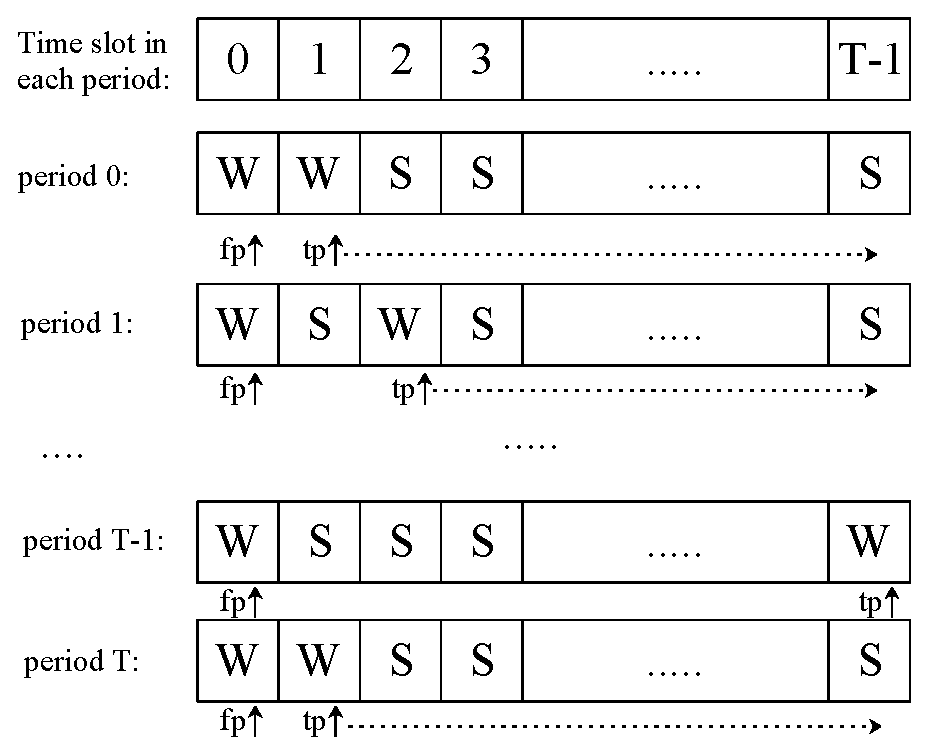
\includegraphics[width=2.5in]{./Figure/TP}
\caption{An Sketch of TP construction in Alg. \ref{P-ND}}
\label{TP}
\end{figure}

%The correctness proof of the construction and the time bound analysis
We give a correctness proof of the time 
bound to achieve neighbor discovery process as following:


\begin{theorem}
\label{PBND1}
Alg. \ref{P-ND} guarantees the discovery latency
to be bounded within $O(\frac{nlogn}{\theta_i\theta_j})$ w.h.p.,
where $\theta_i$ and $\theta_j$ are the duty circles of 
a pair of neighbors (node $i$,node$j$) respectively.
\end{theorem}



\begin{IEEEproof}
We first prove that any pair of nodes (node $i$,node$j$) will wake up 
at the same time slot every period $T_iT_j$.

\textbf{Case 1: $T_i \neq T_j$}. Since $T_i$ and $T_j$ are different primes, 
according to Chinese remainder theorem, there exists a time slot $t_\tau \in \lbrack 0,T_iT_j ) $ satisfying:
\begin{equation}
\label{case1.1}
0 = t_\tau  \quad mod \quad  T_i.
\end{equation}
\begin{equation}
\label{case1.2}
\delta = t_\tau  \quad mod \quad  T_j.
\end{equation}
where $\delta$ is the asynchronous drift between node $i$ and node $j$.

Equation\ref{case1.1} and \ref{case1.2}  implies there exists a fixed pointer of node $i$ 
and a fixed pointer of node $j$ rendezvous in every $T_iT_j$  .

\textbf{Case 2: $T_i = T_j$}. Since $T_i = T_j = T$, if the asynchronous drift between 
node $i$ and node $j$ $\delta = 0$, the fixed pointers of node $i$ and node $j$ will 
rendezvous with each other in every period $T$.
Otherwise since the traversing point will traverse all the time slots once during period $(T-1)T$,
there exists a traversing point of node $i$ rendezvous with a fixed pointer
of node $j$ every period $(T-1)T$, and a traversing point of node $j$ 
will consequentially rendezvous with a fixed pointer
of node $i$ once every period $(T-1)T$ as well.

Thus for any pair of neighbor (node $i$, node $j$), they can wake up
at the same time slot at least once in every period $T_iT_j$. Regarding 
the whole period $T_iT_j$ as a time slot in Alg. \ref{Alano}, we obtain the latency 
bound as $O(\frac{nlogn}{\theta_i\theta_j})$.
\end{IEEEproof}




